%# -*- coding:utf-8 -*-
\documentclass[10pt,aspectratio=169,mathserif]{beamer}		

\usepackage{zju}
\usepackage{amsmath,amsfonts,amssymb,bm}
\usepackage{color}
\usepackage{graphicx,hyperref,url}
\usepackage{metalogo}
% \usepackage{fontspec}
\usepackage{mathptmx}
\usepackage{times}
\usepackage{textcomp}
\usepackage{subcaption}
\usepackage{filecontents}
\usepackage[style=verbose,backend=biber]{biblatex}
\usepackage{relsize}
\usepackage{xspace}
\usepackage{booktabs}
\usepackage{pifont}
\usepackage{fontawesome}
\usepackage{bbding}

\addbibresource{ref.bib}

\newcommand{\code}[1]{\texttt{{\detokenize{#1}}}}
\newcommand{\name}{{\texorpdfstring{D{\smaller MA}A{\smaller UTH}}\xspace}\xspace}
\newcommand{\checkcross}{\ding{51}\kern-0.65em\ding{55}}

\usefonttheme{serif}

\beamertemplateballitem

\title{\name: A Lightweight Pointer Integrity-based Secure Architecture to Defeat DMA Attacks}

% \subtitle{Subtitle}			

\author{\textbf{Xingkai Wang}, Wenbo Shen, Yujie Bu, Jinmeng Zhou, Yajin Zhou}
  
\institute{Zhejiang University}

\date{\today{}}
  
\begin{document}

\begin{frame}
	\titlepage
\end{frame}

% \section{Outline}
\begin{frame}{Outline}
	\tableofcontents
\end{frame}

\section{Motivation}
\begin{frame}{Motivation}
	\begin{figure}
		\centering
		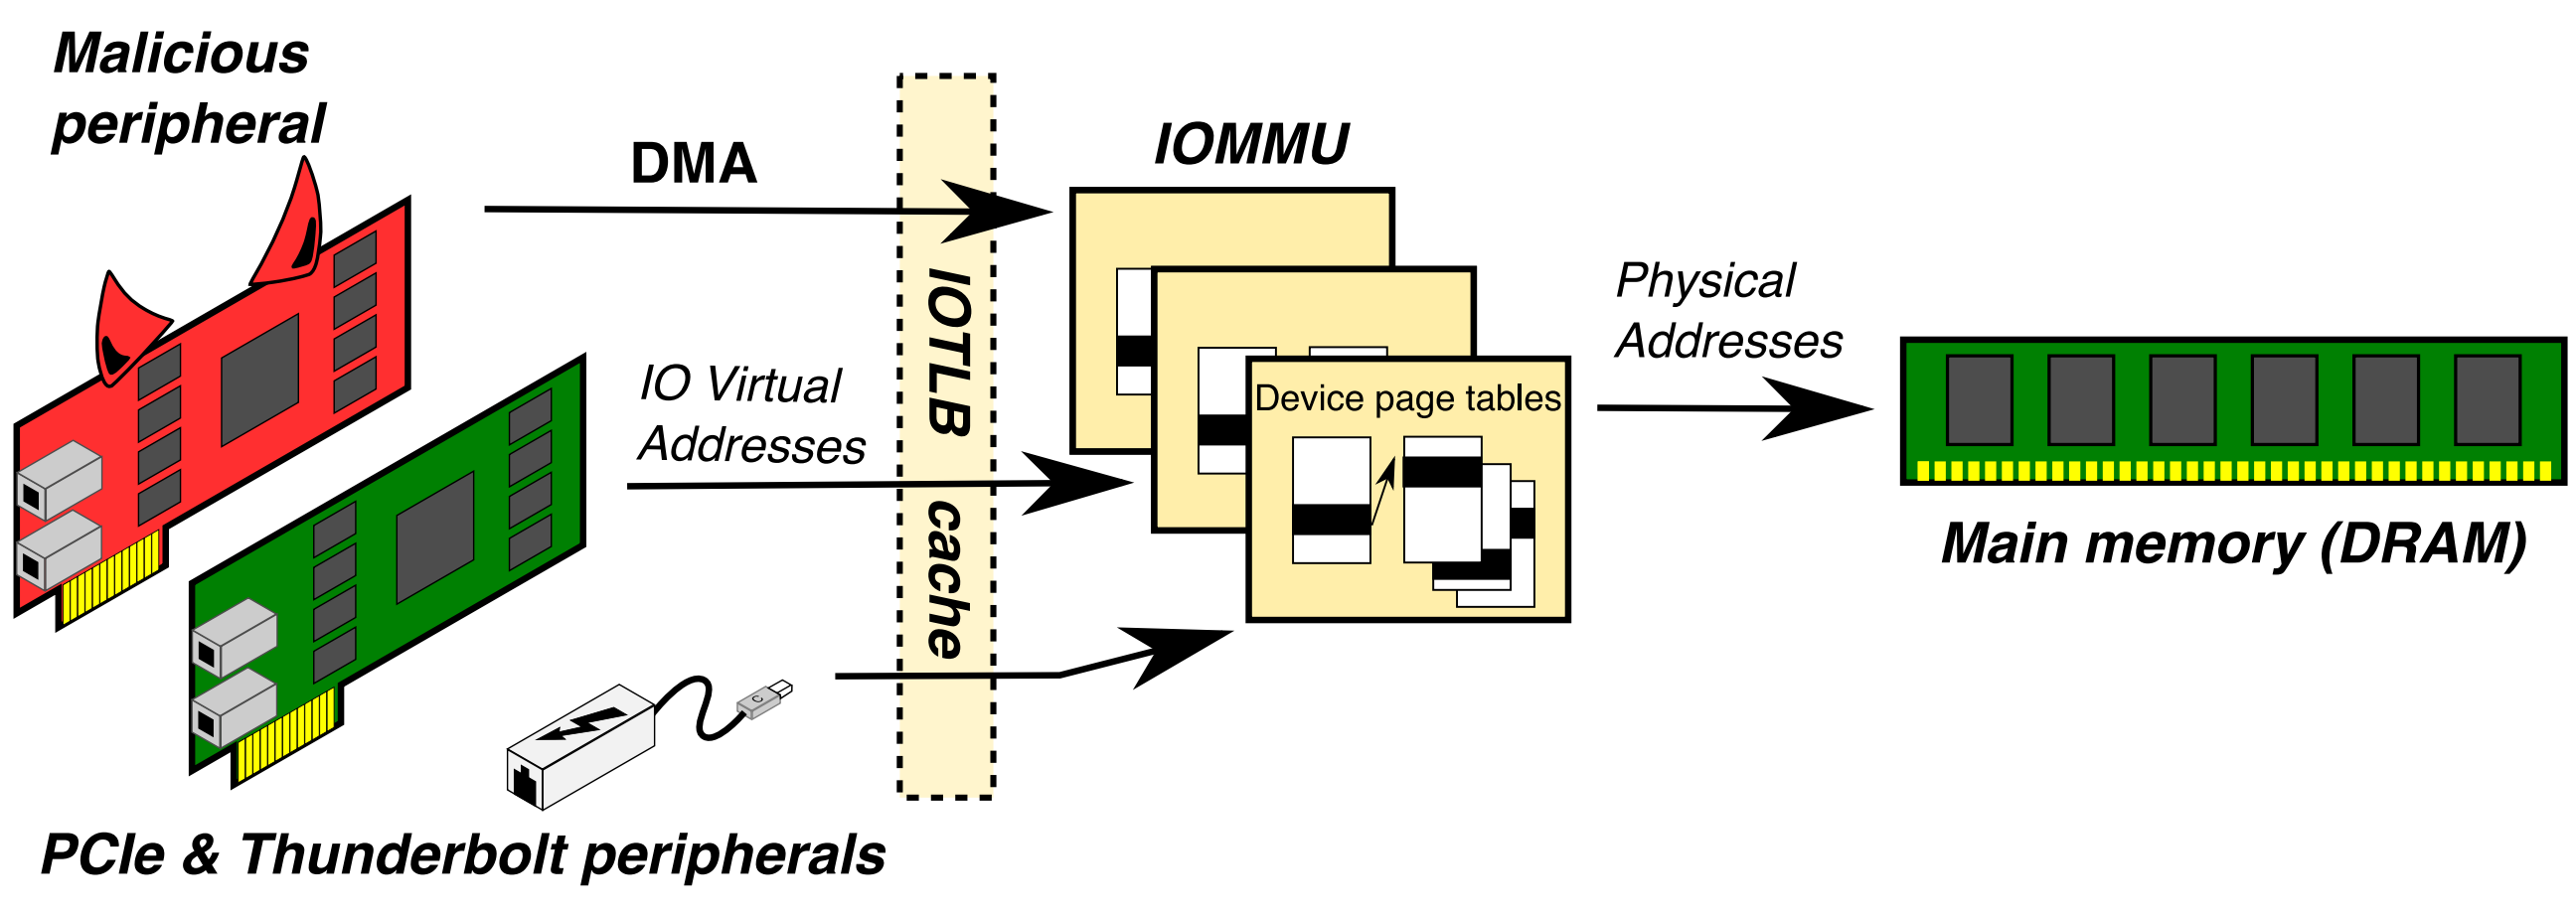
\includegraphics[width=\linewidth]{./images/motivation.png}
		\caption{Some peripherals (or the software running on them) should not be trusted.\footcite{thunderclap}}
	\end{figure}
\end{frame}

\section{Background}

\begin{frame}{Temporal Vulnerability}
	\begin{figure}
		\centering
		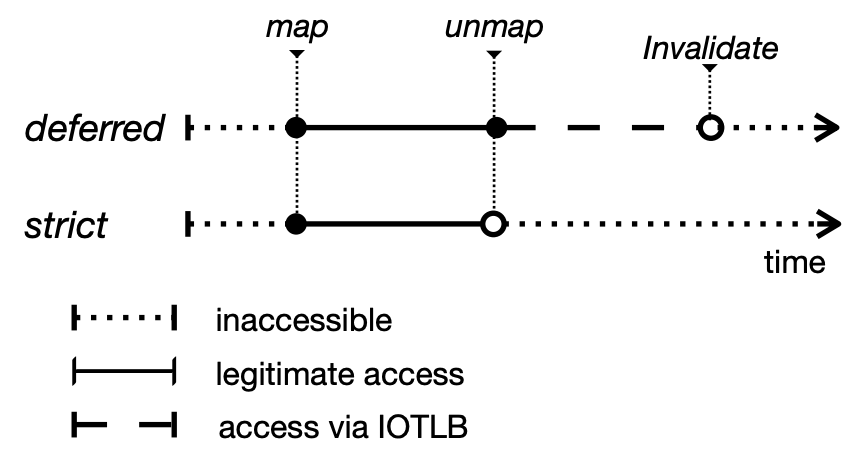
\includegraphics[width=0.6\linewidth]{./images/temporal.png}
		\caption{Peripherals can still access the memory after unmapping. Even if the kernel validates these memory regions after unmapping, the peripherals can still tampers with these regions.\footcite{char}}
	\end{figure}
\end{frame}


\begin{frame}{Spatial Vulnerability}
	\begin{figure}
		\centering
		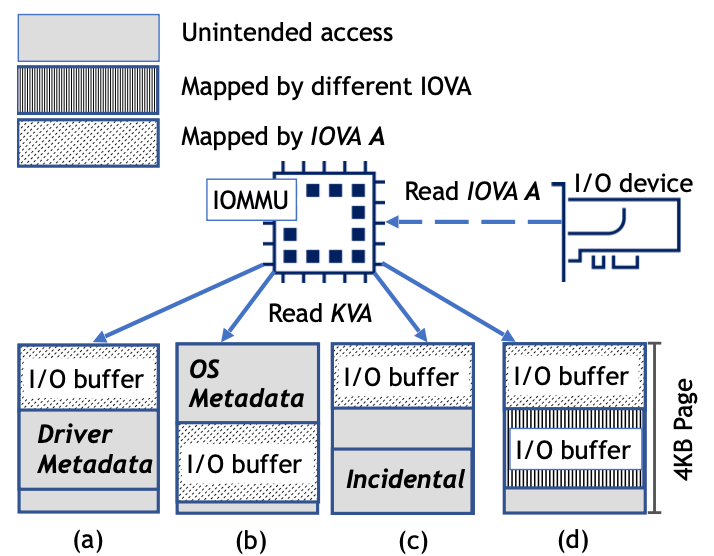
\includegraphics[width=0.52\linewidth]{./images/spatial.png}
		\caption{Page-granularity protection is not enough. Perihperals can still access the memory not for DMA.}
	\end{figure}	
\end{frame}

\begin{frame}{Existing Mechanism}
	\begin{figure}
		\centering
		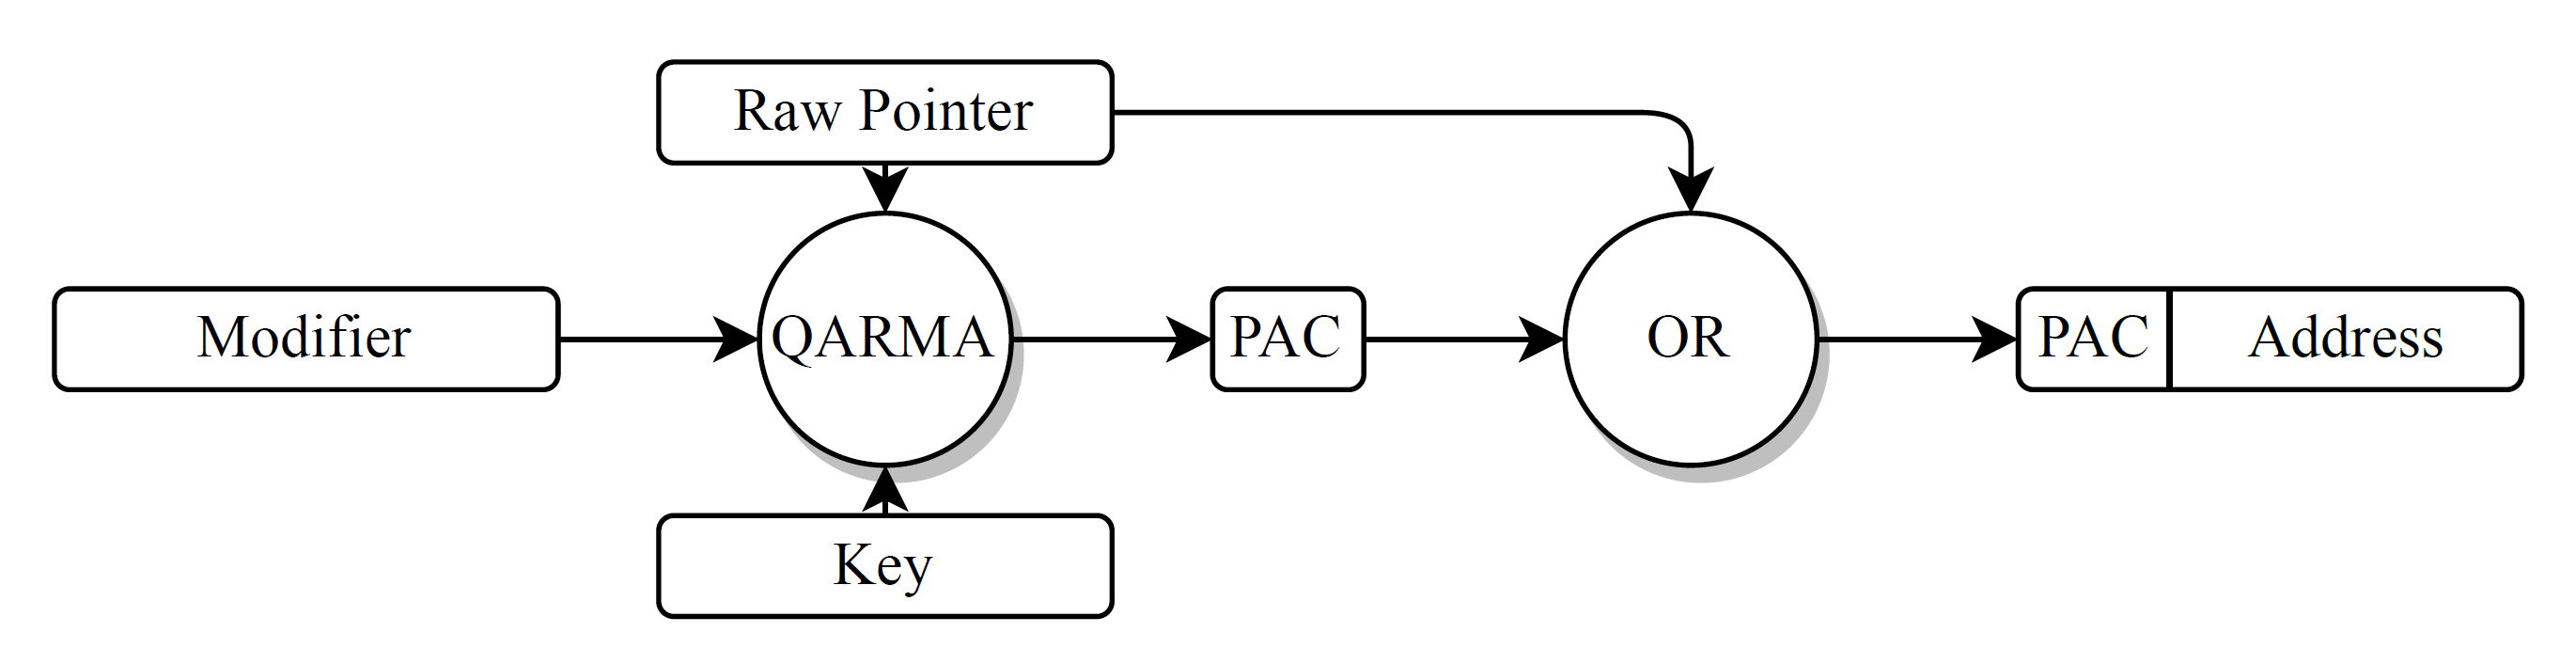
\includegraphics[width=0.9\linewidth]{./images/pa.png}
		\caption{ARM Pointer Authentication. Sign the pointer with a key to prevent attackers from forging pointers.}
	\end{figure}
	But PA cannot prevent dangling pointer reusing (temporal DMA vulnerability), and doesn't support pointer arithmetic (adding offset to pointers).
\end{frame}

\section{Characterization}
\begin{frame}{Characterization}
	\begin{figure}
		\centering
		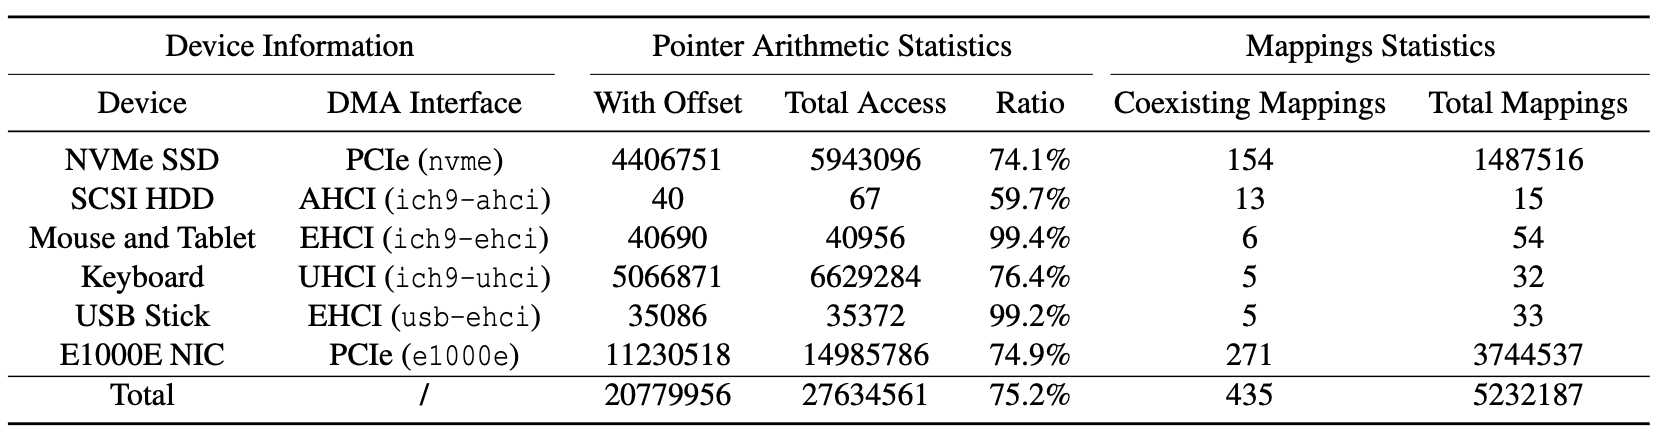
\includegraphics[width=\linewidth]{./images/char.png}
		\caption{Pointer arithmetic is very common on DMA peripherals. This prevents us from using PA.}
	\end{figure}

\end{frame}

\section{Design}
\begin{frame}{Overview}
	\begin{figure}
		\centering
		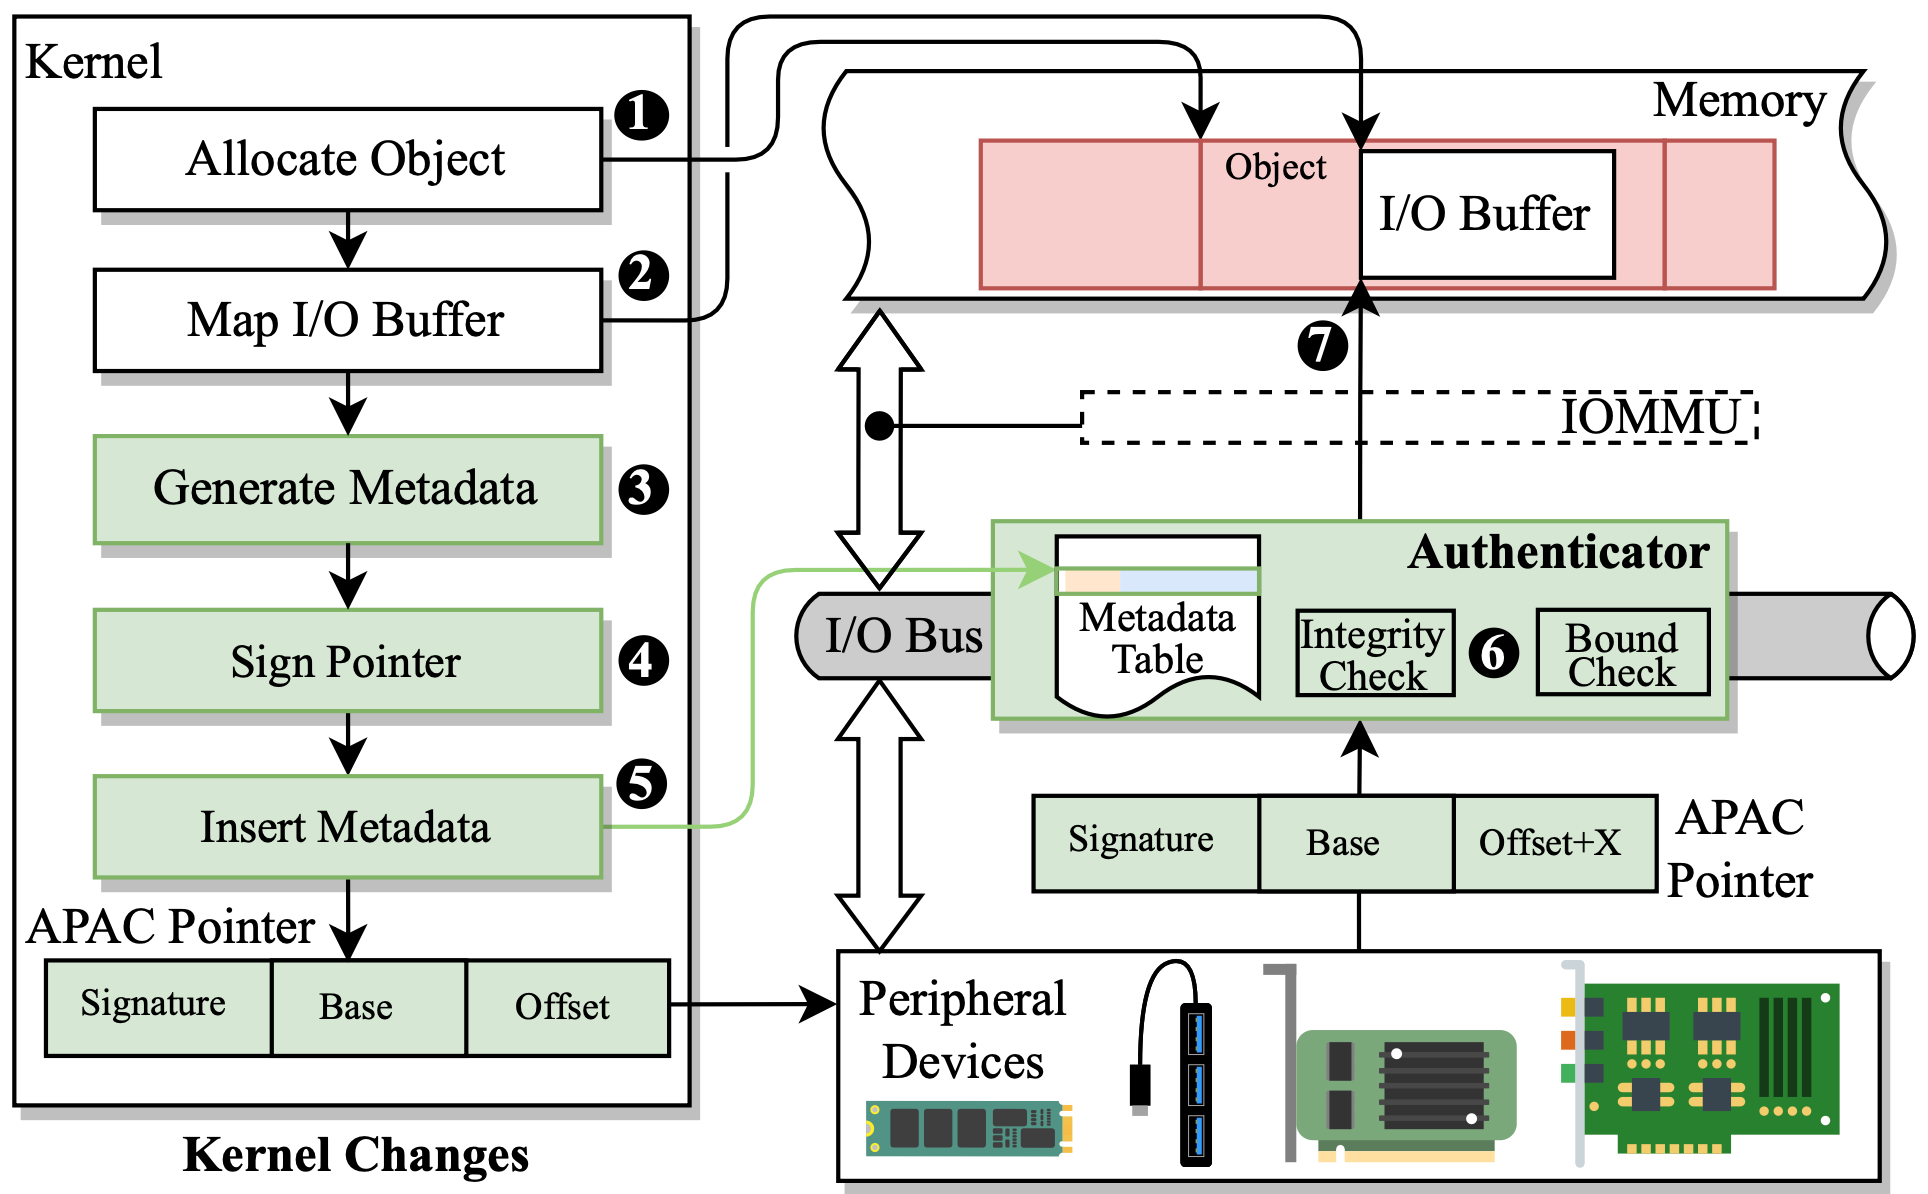
\includegraphics[width=0.6\linewidth]{./images/overview.png}
		\caption{\name sign the DMA pointers in kernel, and authenticate them with hardware on the I/O bus. I.e. Sign with software, authenticate with hardware, forming a software-hardware co-design.}
	\end{figure}	
\end{frame}

\begin{frame}{Partial Authentication}
	\begin{figure}
		\centering
		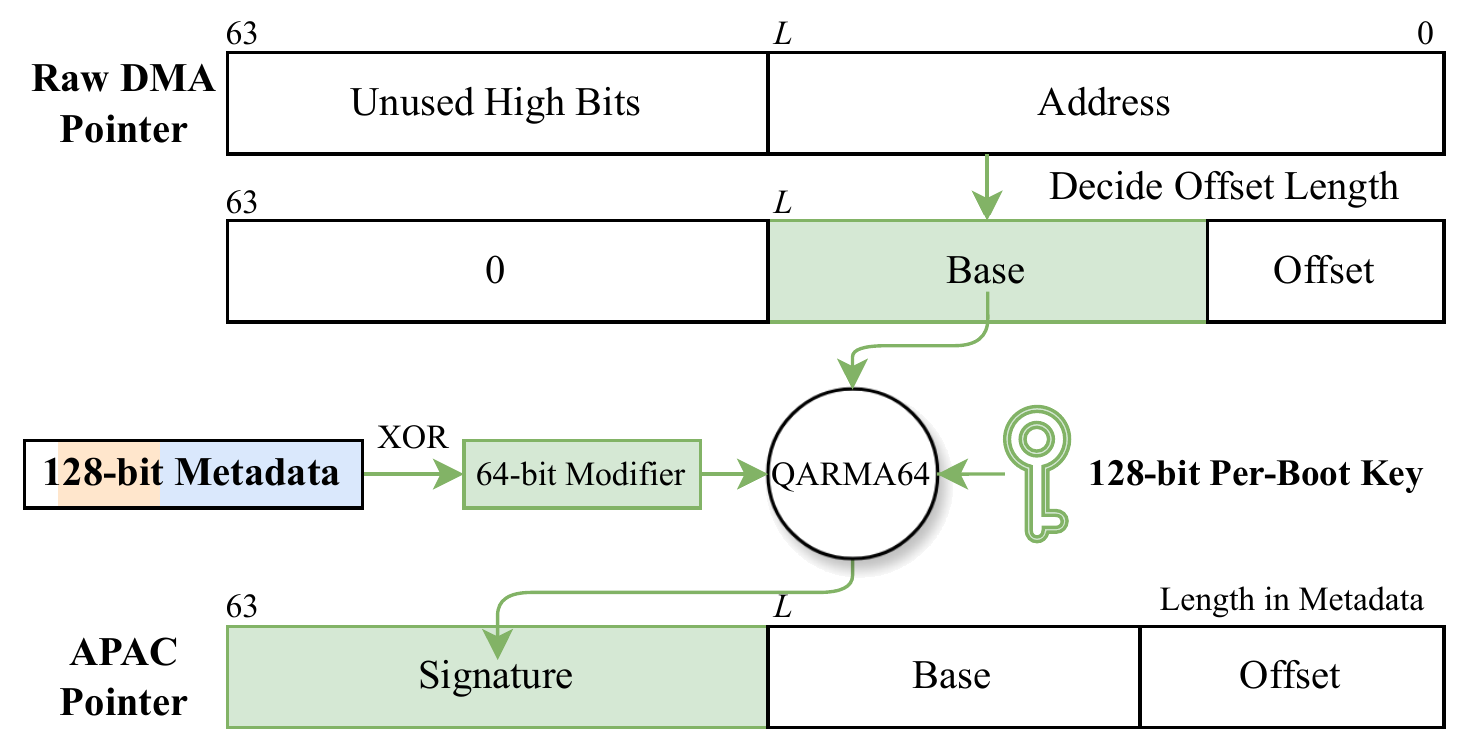
\includegraphics[width=0.7\linewidth]{./images/apac.png}
		\caption{The signature of the pointer is calculated with the \textit{base}, the \textit{metadata} generated at mapping time, and the encryption \textit{key}. The \textit{offset} bits are not used for pointer authentication, thus supporting pointer arithmetic.}
	\end{figure}
\end{frame}

\begin{frame}{Partial Authentication (cont.)}
	\begin{figure}
		\centering
		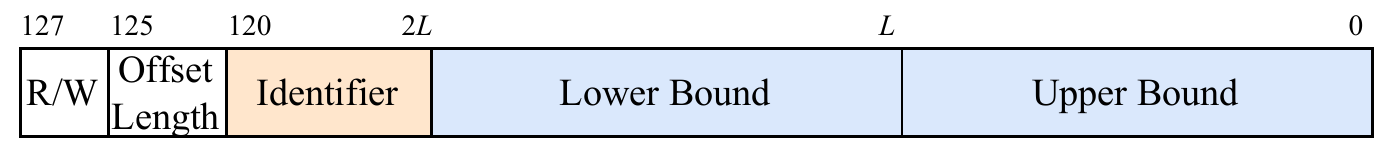
\includegraphics[width=0.6\linewidth]{./images/metadata.png}
		\caption{Metadata format. The metadata is stored in a dedicated storage to authenticate the DMA transactions. The index of the metadata is the same as the signature.}
	\end{figure}
	\vspace{-20pt}
	\begin{figure}
		\centering
		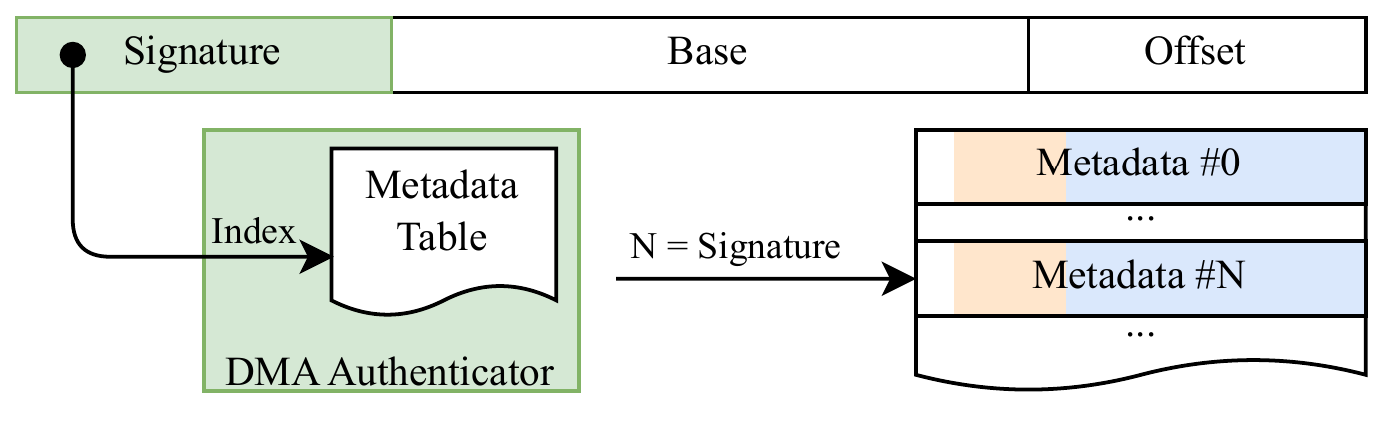
\includegraphics[width=0.6\linewidth]{./images/signing.png}
		\caption{When the DMA reaches the I/O bus, the hardware authenticates the DMA transaction with the metadata. The metadata is located with the signature on the DMA pointer.}
	\end{figure}
\end{frame}

\section{Implementation}
\begin{frame}{Architecture}
	\begin{figure}
		\centering
		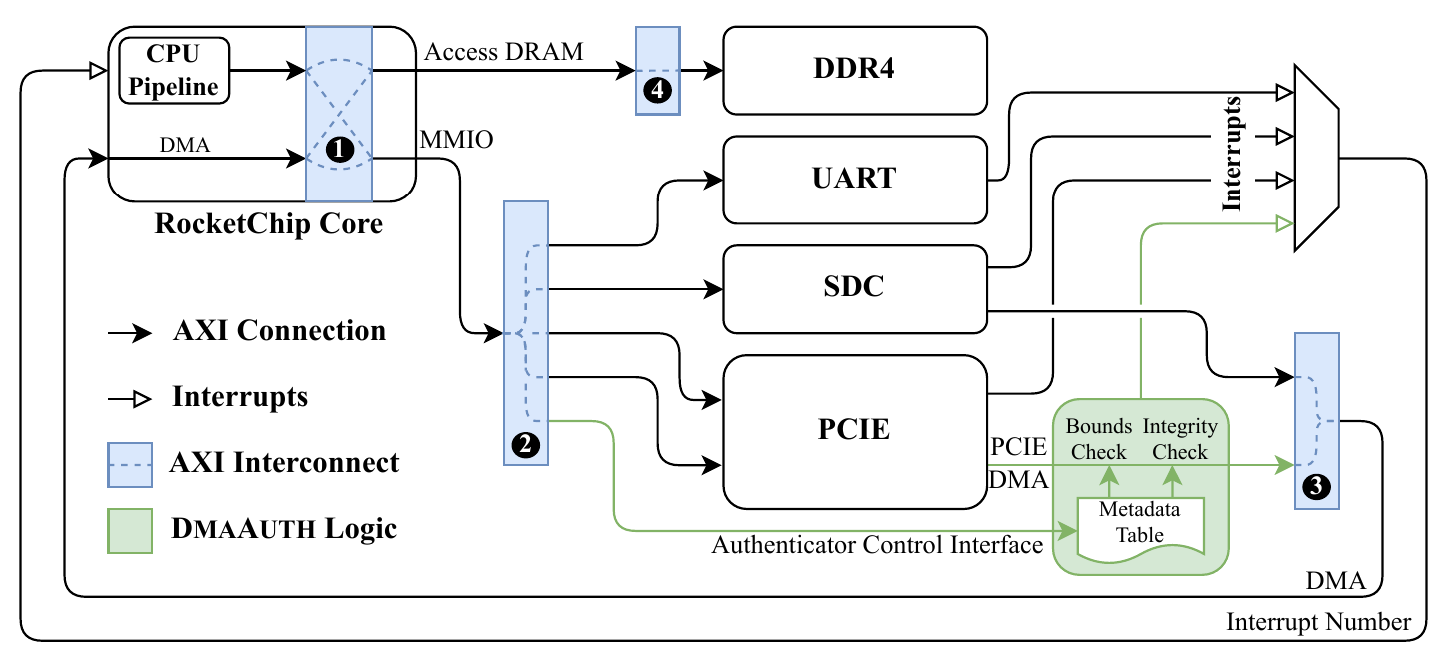
\includegraphics[width=0.82\linewidth]{./images/implementation.png}
		\caption{The hardware architecture of \name. The extra hardware is responsible for authenticating all the DMA transactions from PCIe bus.}
	\end{figure}	
\end{frame}

\begin{frame}{Actual Hardware}
	\begin{figure}
		\centering
		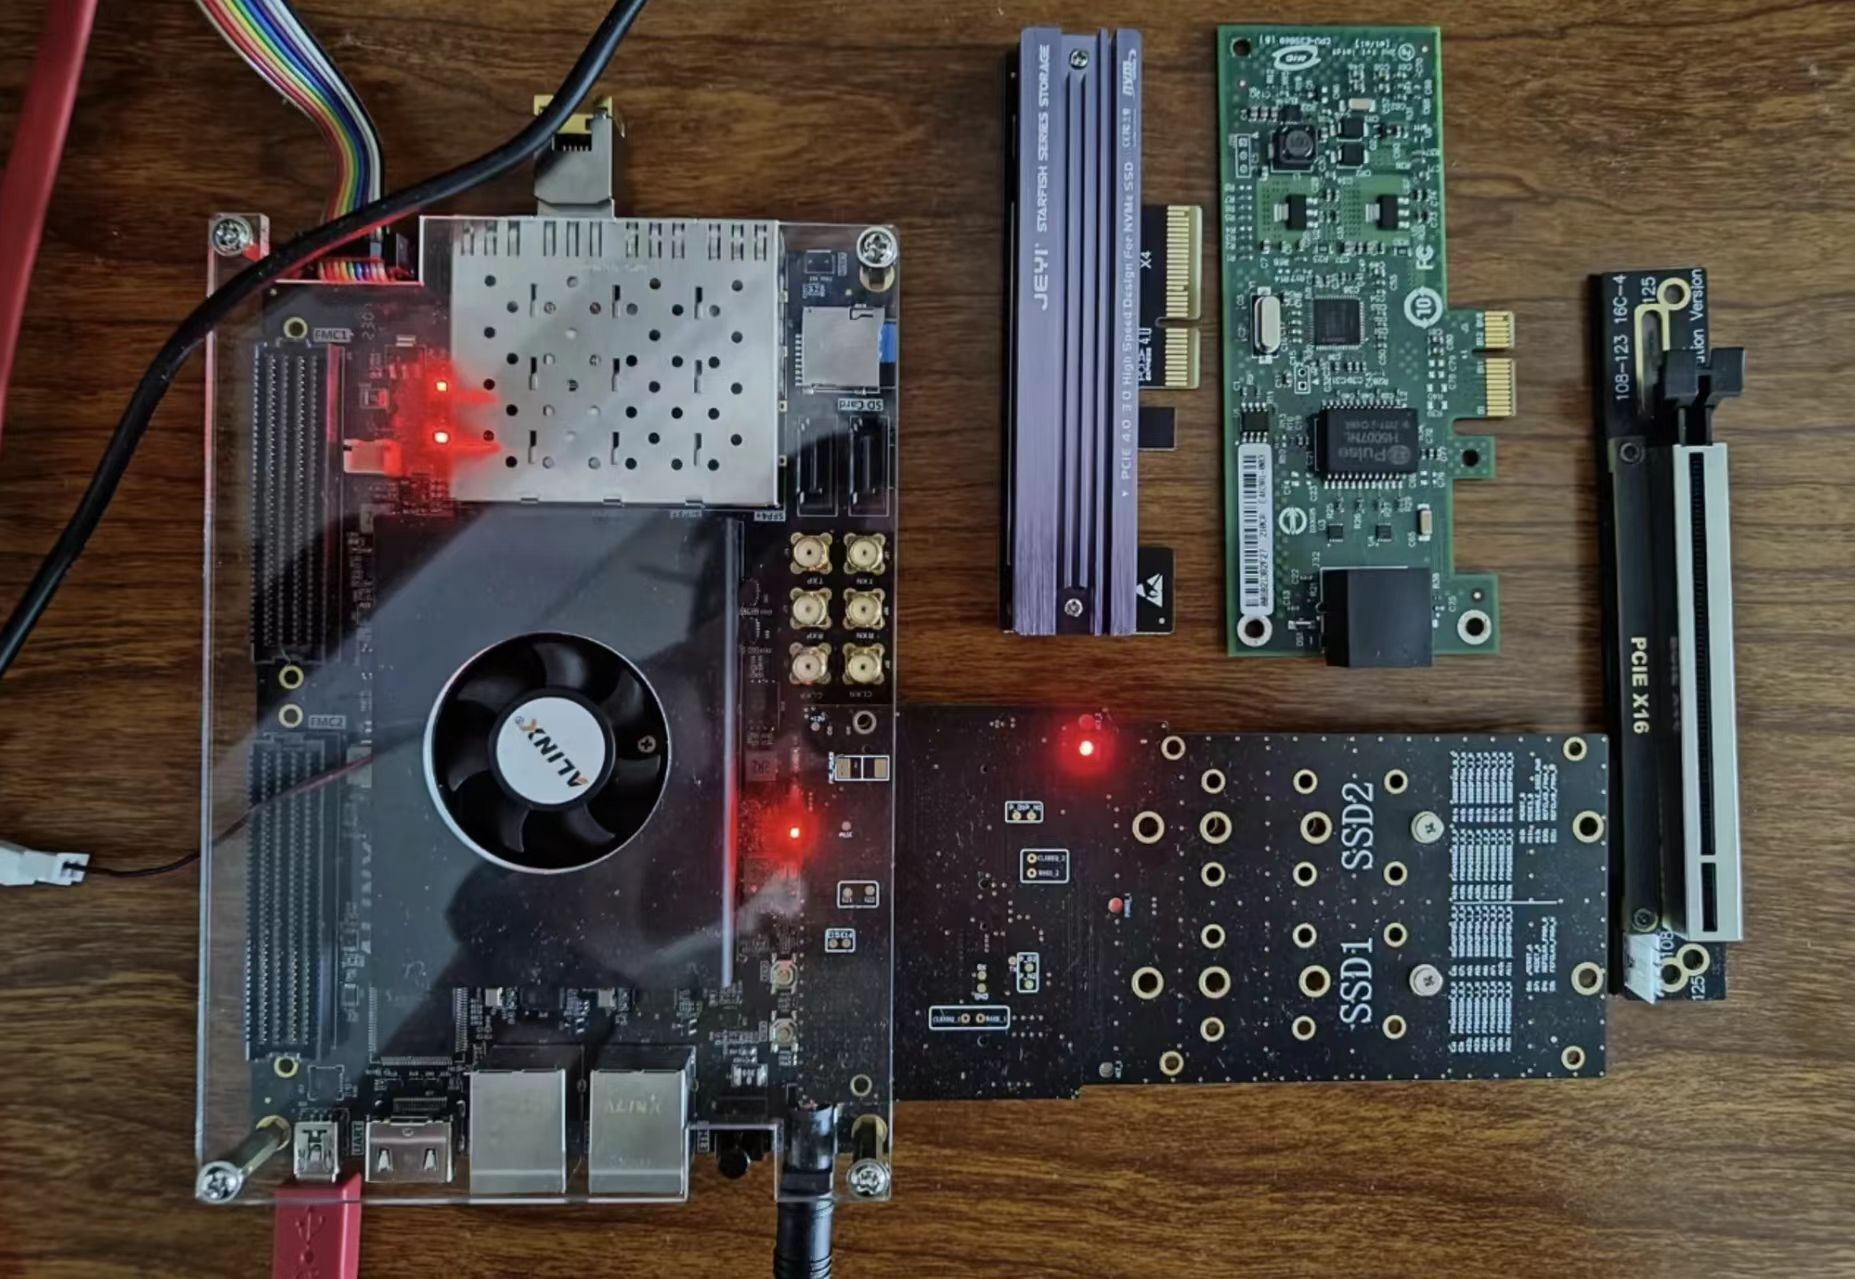
\includegraphics[width=0.58\linewidth]{./images/actual.jpg}
		\caption{\name is implemented on a XCKU040 FPGA with PCIe Gen3 x8 support.}
	\end{figure}
\end{frame}

\section{Evaluation}

\begin{frame}{Security Evaluation}
	\begin{table}[t!]
	\centering
	% \scriptsize
	%   \caption{Security evaluation.}
	% \vspace{-8pt}
	\label{tab:sec}
	\begin{tabular}{lcccccc}
		\toprule
		\multicolumn{2}{c}{Attack Information} & \multicolumn{3}{c}{Security Analysis}\\
		\cmidrule(r){1-2} \cmidrule(l){3-5}
		Attacks & Type & Bare & IOMMU & Ours\\
		\midrule
		\ding{182} Full Memory Dump & Arbitrary Read & \ding{55} & \ding{51} & \ding{51}\\
		\ding{183} Denial of Service & Sub-page Write & \ding{55} & \ding{55} & \ding{51}\\
		\ding{184} Data Pointer Tampering & Sub-page Write & \ding{55} & \ding{55} & \ding{51}\\
		\ding{185} Control Flow Hijack & Sub-page Write & \ding{55} & \ding{55} & \ding{51}\\
		\ding{186} Information Leak & Sub-page Read & \ding{55} & \ding{55} & \ding{51}\\
		\ding{187} Access Unmapped & Temporal & \ding{55} & \checkcross & \ding{51}\\
	\bottomrule
	\vspace{-24pt}
	\end{tabular}
	\end{table}
\end{frame}

\begin{frame}{Performance Evaluation}
	\begin{figure}
		\centering
		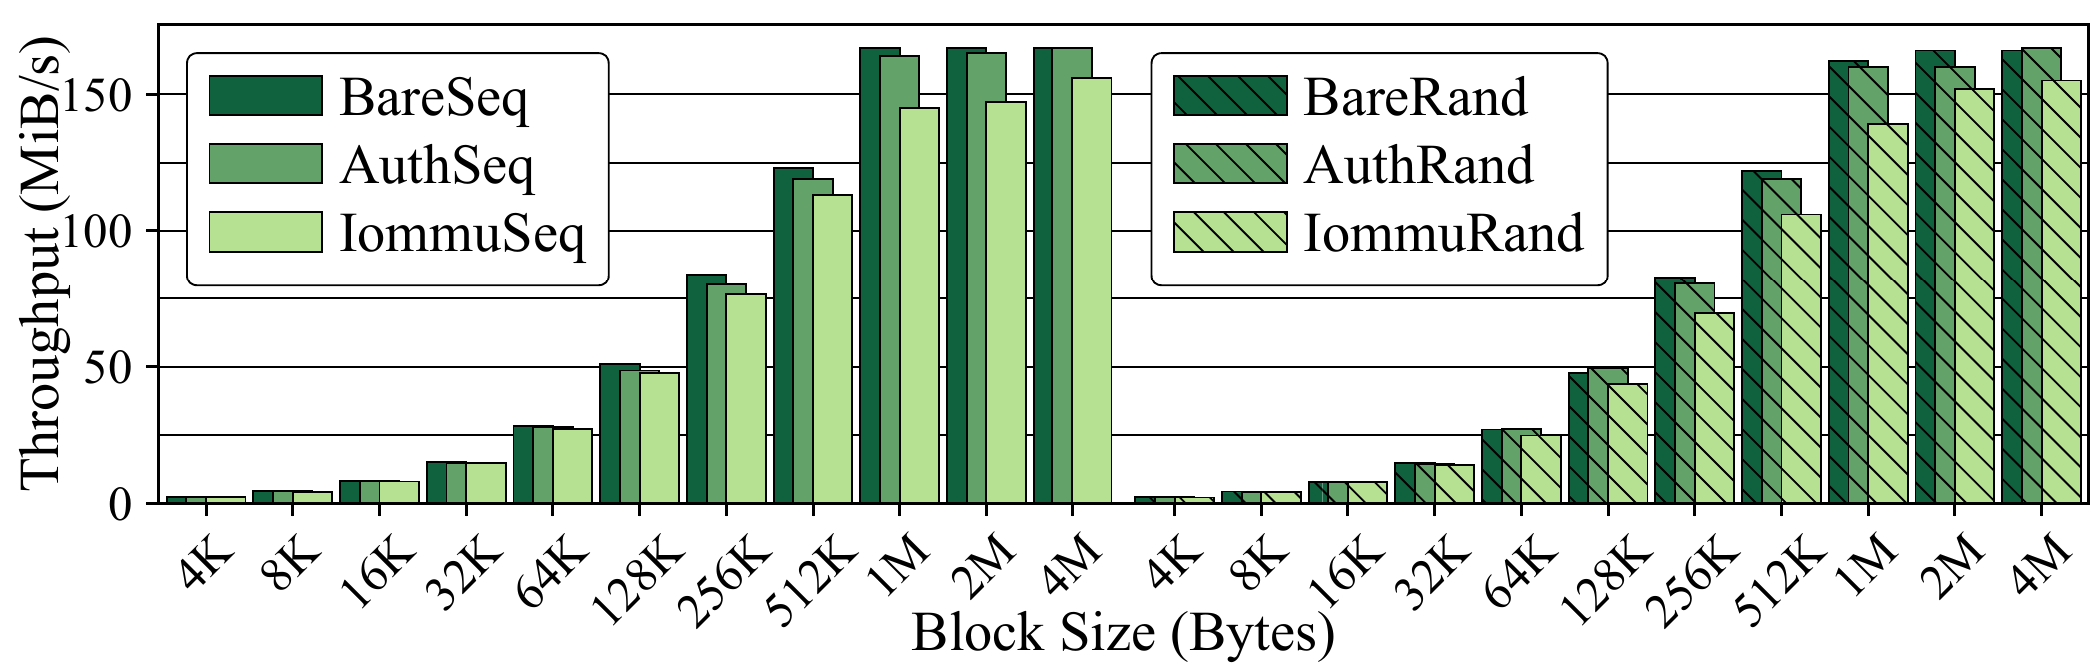
\includegraphics[width=0.63\linewidth]{./images/throughput.png}
	\end{figure}	
	\vspace{-15pt}
	\begin{figure}
		\centering
		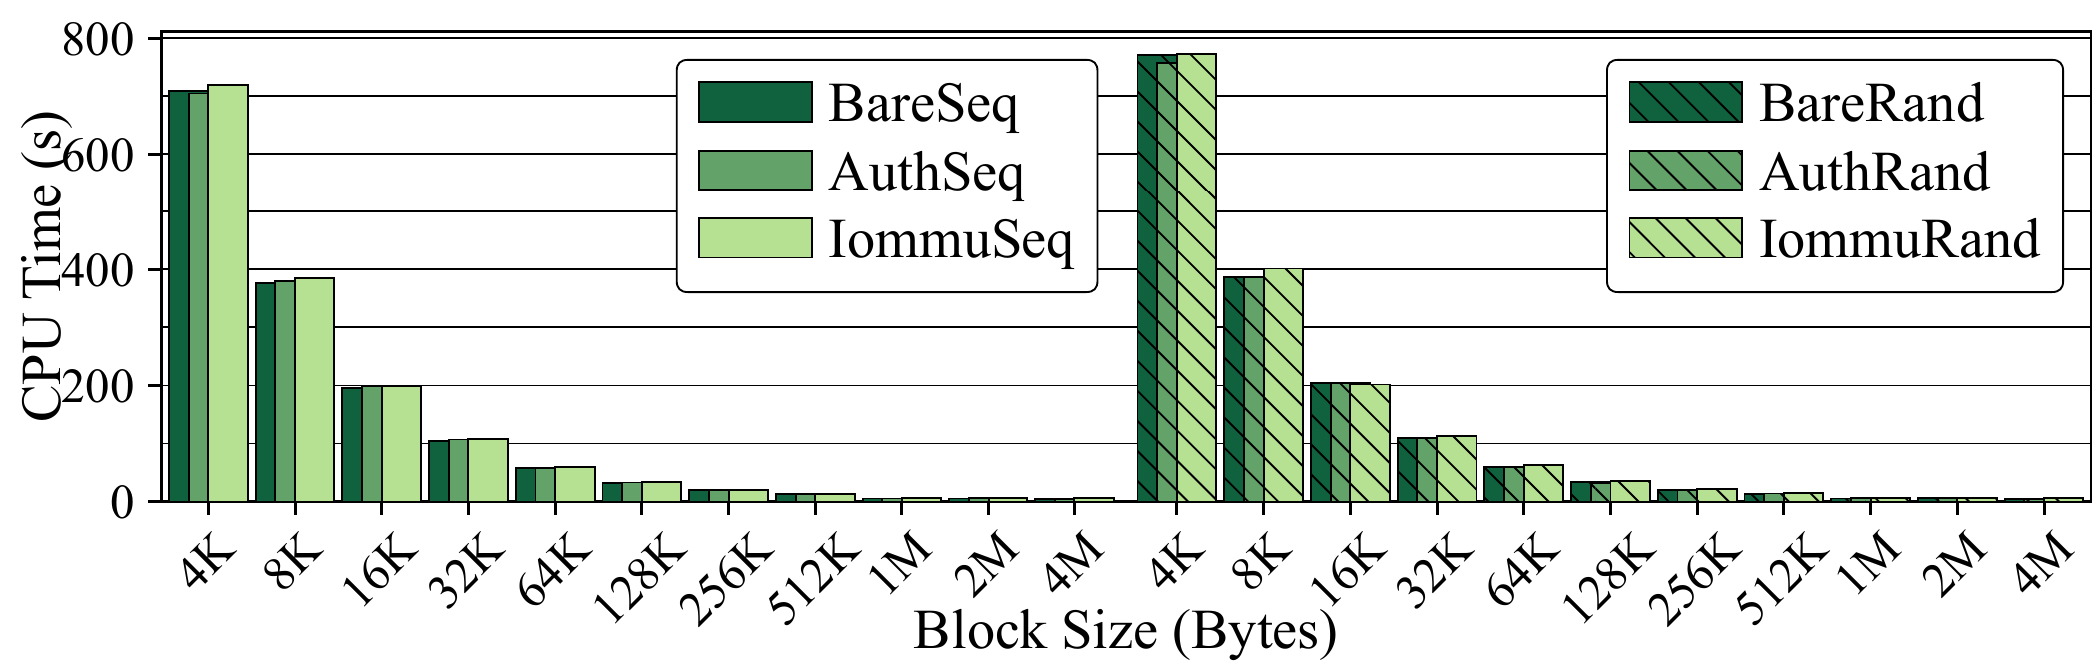
\includegraphics[width=0.63\linewidth]{./images/cputime.png}
		\caption{\name outperforms IOMMU in terms of both throughput and CPU time.}	
	\end{figure}
\end{frame}

% \section{Background}
% \begin{frame}
% 	\frametitle{Existing Mechanisms}
% 	\begin{figure}
% 		\centering
% 		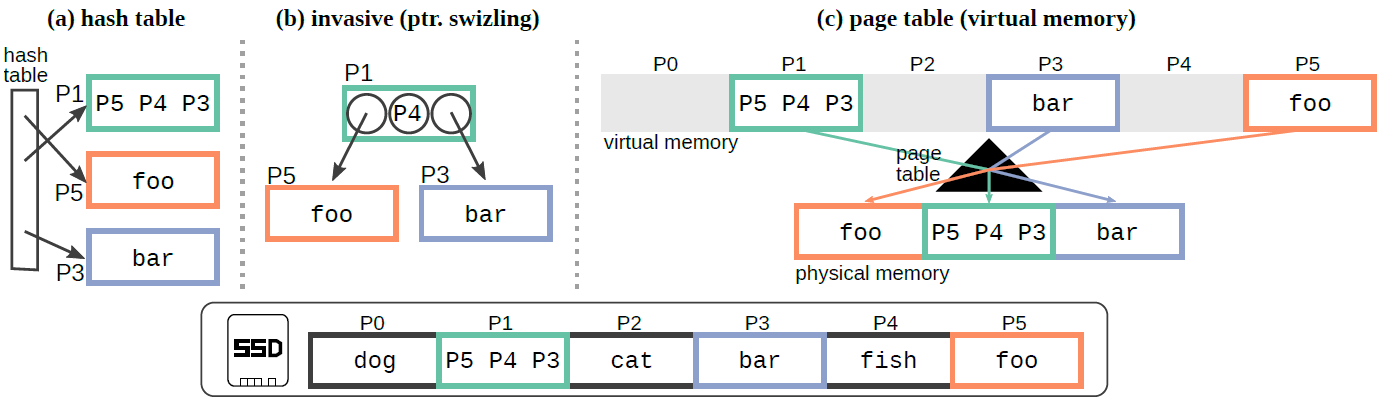
\includegraphics[width=13cm]{./images/existing.png}
% 		\caption{caption}
% 	\end{figure}
% \end{frame}

% \begin{frame}{Design: vmcache (cont.)}
% 	\begin{figure}
% 		\centering
% 		\begin{subfigure}{0.65\linewidth}
% 			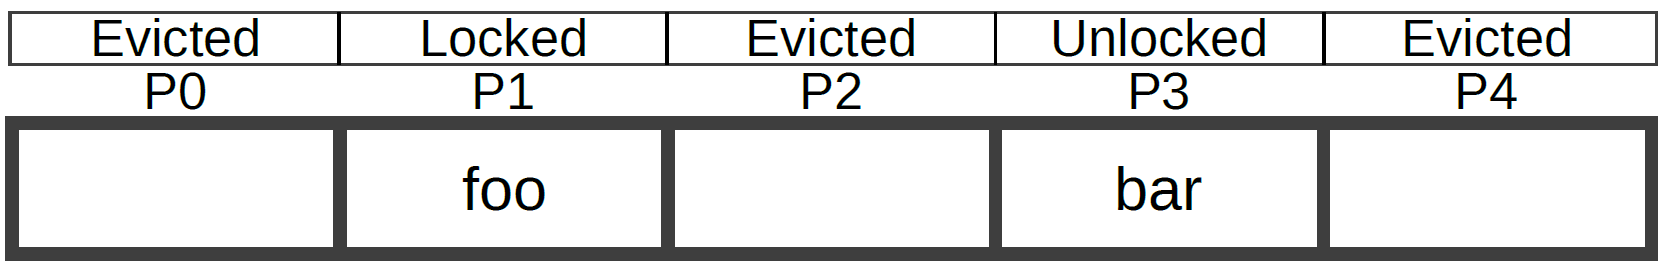
\includegraphics[width=\linewidth]{./images/states.png}
% 			\caption{subcaption}
% 		\end{subfigure}
% 		\begin{subfigure}{0.28\linewidth}
% 			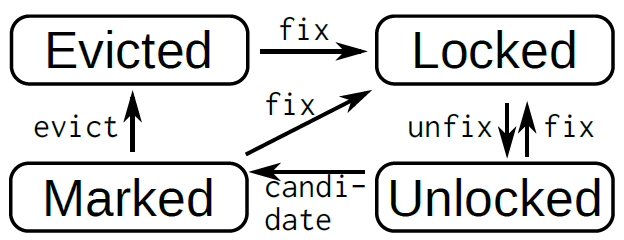
\includegraphics[width=\linewidth]{./images/transfer.png}
% 			\caption{subcaption}
% 		\end{subfigure}
% 		\caption{caption}
% 	\end{figure}
% \end{frame}

% \section{References}
% \begin{frame}{References}
% 	\begin{thebibliography}{99}
% 		\bibitem{zhao1} Yi~Zhao, {\sl An introduction to X}, Sep.~15, 2015
% 		\bibitem{qian2} Er~Qian, San~Sun,
% 		Phys.\ Lett.\ A {\bf xx}, 2xx (20xx)
% 		\bibitem{li4} Si~Li, Phys.\ Rev.\ C {\bf xx}, 5xx (20xx)

% 	\end{thebibliography}
% \end{frame}

\end{document}